\section{积分的定义}
\label{sec:integral-definition}

集合的测度已经能够累计一块区域的大小。现在让每个位置带上一个数值贡献，由函数$f$给出，再问这些贡献的总和是多少。若$f$在一块区域上取常值$c$，这块区域的贡献自然是$c$乘以它的测度；困难在于一般函数在任何区域内都可能不断改变取值。本节先准确计算有限个常值块的贡献，再按函数值分层构造逼近一般函数的简单函数，用“从下方逼近所得累计值的上确界”定义非负函数的积分；随后扩展被积函数的取值范围，最后利用第~\ref{chap:measures}章的Jordan分解定义有符号测度的积分。全节固定一个测度空间$(X,\mathcal A,\mu)$，约定$0\cdot(+\infty)=0$。

\subsection{简单函数的积分}
\label{sec:integral-simple}

\paragraph{有限个常值块的累计}
按定义~\ref{def:measure-simple-function}，简单函数是只取有限多个实数值的可测函数。若非负简单函数$s$取值$c_1,\dots,c_m\ge0$，令$A_i=\{s=c_i\}$，这些集合可测、两两不交且并为$X$，于是$s=\sum_{i=1}^mc_i\mathbf 1_{A_i}$。在$A_i$上每一点的贡献都是$c_i$，这一层的总贡献应为“高度乘以测度”$c_i\mu(A_i)$，再把各层相加。

\begin{definition}[非负简单函数的积分]
\label{def:integral-simple}
设$s=\sum_{i=1}^mc_i\mathbf 1_{A_i}$，其中$c_i\in[0,+\infty)$，$A_1,\dots,A_m\in\mathcal A$两两不交。定义
\[
 \int_Xs\,\mathrm d\mu=\sum_{i=1}^mc_i\,\mu(A_i)\in[0,+\infty].
\]
对$E\in\mathcal A$，定义$s$在$E$上的积分为$\int_Es\,\mathrm d\mu=\int_Xs\mathbf 1_E\,\mathrm d\mu$。
\end{definition}

这里直接使用已有测度$\mu$给各层称重，没有把$s$解释成别的什么东西；积分可以取$+\infty$，例如实轴上$\mathbf 1_{\mathbb R}$对$\lambda$的积分是$\lambda(\mathbb R)=+\infty$。约定$0\cdot(+\infty)=0$保证取值为零的层不贡献任何量，哪怕它的测度无限：在$\mathbb R$上，$s=2\cdot\mathbf 1_{[0,1]}$同时可以写成$2\cdot\mathbf 1_{[0,1]}+0\cdot\mathbf 1_{\mathbb R\setminus[0,1]}$，两种写法给出的积分都应是$2$。

图~\ref{fig:integral-simple-height-measure}中，$[0,3]$上的$s$在$A_1=[0,1)\cup[2,2.5)$上取$2$，在$A_2=[1,2)\cup[2.5,3]$上取$0.5$。两层都由两段区间组成，$\lambda(A_1)=\lambda(A_2)=1.5$，所以$\int_{[0,3]}s\,\mathrm d\lambda=2\times1.5+0.5\times1.5=3.75$。计算时先把取值相同的块合并成一层，再乘以该层的测度；层本身不必是区间，只需可测。

\begin{figure}[!htbp]
 \centering
 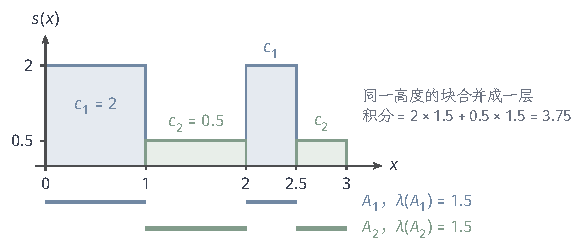
\includegraphics[width=98.771mm]{figures/02-abstract-mathematics/01-metric-and-measure/tikz/c3-simple-height-measure/figure.pdf}
 \caption{简单函数积分的“高度乘以测度”。$[0,3]$上的$s$在$A_1=[0,1)\cup[2,2.5)$（蓝）上取$2$，在$A_2=[1,2)\cup[2.5,3]$（绿）上取$0.5$；下方两行线段标出两层在横轴上占据的集合。积分为$2\times1.5+0.5\times1.5=3.75$。}
 \label{fig:integral-simple-height-measure}
\end{figure}

\paragraph{与表示方式无关}
同一个简单函数可以有多种写法，例如$\mathbf 1_{[0,2]}=1\cdot\mathbf 1_{[0,1]}+1\cdot\mathbf 1_{(1,2]}$，定义~\ref{def:integral-simple}允许任意一种不交写法，因此先要确认结果不依赖写法。办法是把两种写法放到共同的细分上比较。

\begin{lemma}[简单函数积分的良定性与基本运算]
\label{lem:integral-simple-properties}
设$s,t$是非负简单函数，$a\in[0,+\infty)$。
\begin{enumerate}
 \item $\int_Xs\,\mathrm d\mu$不依赖于$s$的不交表示。
 \item $\int_X(s+t)\,\mathrm d\mu=\int_Xs\,\mathrm d\mu+\int_Xt\,\mathrm d\mu$，$\int_Xas\,\mathrm d\mu=a\int_Xs\,\mathrm d\mu$。
 \item 若$s\le t$，则$\int_Xs\,\mathrm d\mu\le\int_Xt\,\mathrm d\mu$。
 \item 集合函数$E\mapsto\int_Es\,\mathrm d\mu$是$(X,\mathcal A)$上的测度。
\end{enumerate}
\end{lemma}

\begin{proof}
设$s=\sum_ic_i\mathbf 1_{A_i}=\sum_jd_j\mathbf 1_{B_j}$是两种不交表示。补上$A_0=X\setminus\bigcup_iA_i$与系数$c_0=0$，它贡献$0\cdot\mu(A_0)=0$，不改变定义中的和；对$B_j$同样处理。于是可设$\{A_i\}$与$\{B_j\}$都是$X$的有限可测分割。由有限可加性，$\mu(A_i)=\sum_j\mu(A_i\cap B_j)$，故
\[
 \sum_ic_i\mu(A_i)=\sum_{i,j}c_i\mu(A_i\cap B_j)=\sum_{i,j}d_j\mu(A_i\cap B_j)=\sum_jd_j\mu(B_j).
\]
中间一步逐项成立：若$A_i\cap B_j\ne\varnothing$，其中一点的函数值同时是$c_i$与$d_j$，故$c_i=d_j$；若交集为空，两边该项都为零。$[0,+\infty]$中有限非负数与和的分配律成立，所以上述运算不涉及无定义的表达式。第1条得证。

对第2条，取$s=\sum_ic_i\mathbf 1_{A_i}$、$t=\sum_jd_j\mathbf 1_{B_j}$为两个分割上的表示。在共同细分上，$s+t=\sum_{i,j}(c_i+d_j)\mathbf 1_{A_i\cap B_j}$是$s+t$的一个不交表示，由第1条
\[
 \int_X(s+t)\,\mathrm d\mu=\sum_{i,j}(c_i+d_j)\mu(A_i\cap B_j)=\int_Xs\,\mathrm d\mu+\int_Xt\,\mathrm d\mu.
\]
数乘只把每个系数乘以$a$。对第3条，在同一细分上，凡$A_i\cap B_j\ne\varnothing$就有$c_i\le d_j$，逐项比较$\sum_{i,j}c_i\mu(A_i\cap B_j)$与$\sum_{i,j}d_j\mu(A_i\cap B_j)$即得。

对第4条，$\int_Es\,\mathrm d\mu=\sum_ic_i\mu(A_i\cap E)$。每个$E\mapsto\mu(A_i\cap E)$都是测度：$E_n$两两不交时$A_i\cap E_n$也两两不交，可数可加性直接继承。有限个测度的非负系数组合仍是测度（引理~\ref{lem:measure-weighted-sum}），结论成立。
\end{proof}

第4条在区域之间比较累计值：$E\subseteq F$时$\int_Es\le\int_Fs$，递增区域上的累计值随区域收敛。下一小节以后的下方逼近要反复比较这样的累计值，第~\ref{sec:integral-mct}小节证明单调收敛定理时将用到它的从下连续性。

\subsection{简单函数逼近}
\label{sec:integral-simple-approximation}

\paragraph{按函数值分层}
一般可测函数在一块区域内可能不断改变取值，不能直接用有限个常值贡献精确累计。黎曼积分的做法是把定义域切成小区间，在每段上取一个代表值；这要求定义域是区间，也要求函数在小区间上变化不大。测度空间$X$上未必有“小区间”，可测函数也可能处处剧烈振荡。另一种做法是切分\emph{函数值}：把取值范围分成若干层，收集函数值落在同一层的全部点。这样的点集是阈值集合的差，对可测函数总是可测的，不论$X$是什么空间。图~\ref{fig:integral-riemann-lebesgue-partitions}对比了两种切法：同一层$\{f\ge1.5\}$在横轴上由两段不相邻的区间组成，测度只需把它们的长度相加。

\begin{figure}[!htbp]
 \centering
 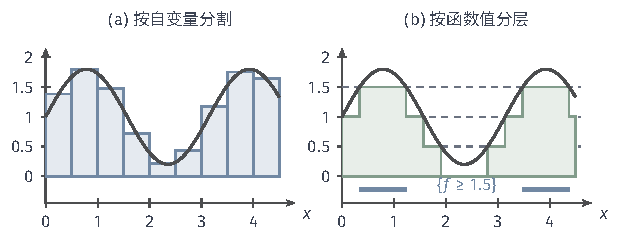
\includegraphics[width=104.881mm]{figures/02-abstract-mathematics/01-metric-and-measure/tikz/c3-riemann-lebesgue-partitions/figure.pdf}
 \caption{两种切分方式，$f(x)=1+0.8\sin2x$，$x\in[0,4.5]$。(a)把定义域等分为$9$段，每段取中点值作高度，这是黎曼和的做法。(b)把函数值按步长$0.5$分层，绿色阶梯是$0.5\lfloor2f\rfloor$；最高一层$\{f\ge1.5\}=[0.3376,1.2332)\cup[3.4792,4.3749)$（底部蓝色线段）由两段区间组成，总长约$1.79$。}
 \label{fig:integral-riemann-lebesgue-partitions}
\end{figure}

\begin{lemma}[简单函数逼近]
\label{lem:integral-simple-approx}
设$f:X\to[0,+\infty]$可测。令
\[
 s_n=2^{-n}\bigl\lfloor2^n\min\{f,n\}\bigr\rfloor,\qquad n=1,2,\dots.
\]
则每个$s_n$是非负简单函数，$0\le s_1\le s_2\le\cdots\le f$，且对每个$x\in X$有$s_n(x)\to f(x)$。若$f\le M$有界，则当$n\ge M$时$\sup_X(f-s_n)\le2^{-n}$，即$s_n$一致收敛到$f$。
\end{lemma}

\begin{proof}
\emph{$s_n$是简单函数。}若$f(x)\ge n$，则$\min\{f(x),n\}=n$，$s_n(x)=n$；若$f(x)<n$，则$s_n(x)=k2^{-n}$，其中$k=\lfloor2^nf(x)\rfloor\in\{0,1,\dots,n2^n-1\}$。所以
\[
 s_n=\sum_{k=0}^{n2^n-1}k2^{-n}\mathbf 1_{A_{n,k}}+n\mathbf 1_{\{f\ge n\}},\qquad A_{n,k}=\{k2^{-n}\le f<(k+1)2^{-n}\}.
\]
$A_{n,k}=\{f\ge k2^{-n}\}\setminus\{f\ge(k+1)2^{-n}\}$是两个阈值集合之差，可测；各集合两两不交，$s_n$只取有限多个值。

\emph{递增且不超过$f$。}由$\lfloor y\rfloor\le y$得$s_n\le\min\{f,n\}\le f$。对任意$y\ge0$，$2\lfloor y\rfloor$是不超过$2y$的整数，所以$2\lfloor y\rfloor\le\lfloor2y\rfloor$。记$m_n=\min\{f,n\}\le m_{n+1}$，则
\[
 s_n=2^{-(n+1)}\cdot2\lfloor2^nm_n\rfloor\le2^{-(n+1)}\lfloor2^{n+1}m_n\rfloor\le2^{-(n+1)}\lfloor2^{n+1}m_{n+1}\rfloor=s_{n+1}.
\]

\emph{逐点收敛。}若$f(x)=+\infty$，则$s_n(x)=n\to+\infty$。若$f(x)<+\infty$，当$n>f(x)$时$m_n(x)=f(x)$，由$\lfloor y\rfloor>y-1$得$0\le f(x)-s_n(x)<2^{-n}$。若$f\le M$，这个估计对$n\ge M$在全部$x$上同时成立：$n=M$而$f(x)=n$时差为零，其余情形差小于$2^{-n}$。
\end{proof}

图~\ref{fig:integral-dyadic-approximation}对$[0,2]$上的$f(x)=x^2$画出$s_1$与$s_2$。$n=1$时取值步长为$1/2$、高度截断于$1$，断点在$x=\sqrt{1/2}\approx0.7071$与$x=1$；$n=2$时步长缩为$1/4$、截断高度升到$2$，断点为$\sqrt{k/4}$，$k=1,\dots,8$。每增加一步，既把已有的层对半细分，又把截断线抬高一格，所以逼近从两个方向同时改进：细分处理函数值的细节，截断线的上升处理函数的大值。分层发生在函数值上，断点的位置由$f$决定，而不是事先在定义域上取定。

\begin{figure}[!htbp]
 \centering
 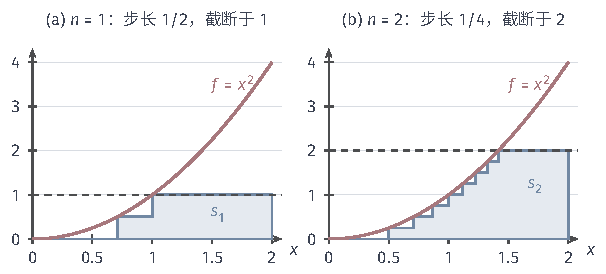
\includegraphics[width=102.634mm]{figures/02-abstract-mathematics/01-metric-and-measure/tikz/c3-dyadic-approximation/figure.pdf}
 \caption{二进分层逼近$f(x)=x^2$，$x\in[0,2]$。蓝色阶梯是$s_n=2^{-n}\lfloor2^n\min\{f,n\}\rfloor$，虚线是截断高度$n$。(a)$n=1$，$s_1$取值$0,0.5,1$；(b)$n=2$，$s_2$取值$0,0.25,\dots,2$，断点为$\sqrt{k/4}$。阶梯始终位于曲线下方，且随$n$增大而升高。}
 \label{fig:integral-dyadic-approximation}
\end{figure}

\paragraph{取正负值的函数}
可正可负的实值可测函数$f$不能直接套用上面的分层，因为下取整会把负值推得更负。把正值部分与负值部分分开处理即可。

\begin{definition}[正部与负部]
\label{def:integral-positive-negative-parts}
对可测函数$f:X\to[-\infty,+\infty]$，称$f^+=\max\{f,0\}$为$f$的\term{正部}（positive part），$f^-=\max\{-f,0\}$为$f$的\term{负部}（negative part）。
\end{definition}

由定理~\ref{thm:measure-function-operations}，$f^+$、$f^-$都是非负可测函数，且
\[
 f=f^+-f^-,\qquad |f|=f^++f^-.
\]
在每一点至多有一个部分非零：$f(x)>0$时$f^-(x)=0$，$f(x)<0$时$f^+(x)=0$。负部取的是$-f$的正值，所以它本身非负。图~\ref{fig:integral-positive-negative-parts}以$f=\sin x$为例：$f^+$在$[0,\pi]$上等于$\sin x$，$f^-$在$[\pi,2\pi]$上等于$-\sin x$，两者都画在横轴上方。

\begin{figure}[!htbp]
 \centering
 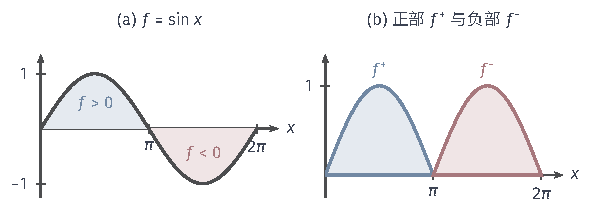
\includegraphics[width=100.034mm]{figures/02-abstract-mathematics/01-metric-and-measure/tikz/c3-positive-negative-parts/figure.pdf}
 \caption{正负部分解，$f(x)=\sin x$，$x\in[0,2\pi]$。(a)$f$在$[0,\pi]$上为正（蓝），在$[\pi,2\pi]$上为负（红）。(b)正部$f^+=\max\{f,0\}$与负部$f^-=\max\{-f,0\}$都是非负函数，且$f=f^+-f^-$，$|f|=f^++f^-$。}
 \label{fig:integral-positive-negative-parts}
\end{figure}

对实值可测$f$，分别用引理~\ref{lem:integral-simple-approx}构造$s_n^+\uparrow f^+$与$s_n^-\uparrow f^-$，令$\varphi_n=s_n^+-s_n^-$。它是简单函数，逐点收敛到$f$，并且$|\varphi_n|\le s_n^++s_n^-\le|f|$，即逼近函数始终受$|f|$控制。若$|f|\le M$，因为每点只有一个部分起作用，$n\ge M$时$\sup_X|f-\varphi_n|\le2^{-n}$，逼近是一致的。至此一般可测函数与简单函数之间的逼近关系已经建立；这些逼近函数的积分是否收敛到某个确定的数，要在定义积分以后才能讨论。

\subsection{非负可测函数的积分}
\label{sec:integral-nonnegative}

\paragraph{下方逼近的上确界}
对非负可测函数$f$，位于$f$下方的每个非负简单函数$s$都给出总贡献的一个偏小估计$\int s\,\mathrm d\mu$。上一小节说明这样的$s$能够逐层读出$f$的取值，所以把全部偏小估计的上确界作为积分是合理的。定义并不指定使用哪一条逼近列，这避免了“换一列逼近是否得到同一个数”的问题。

\begin{definition}[非负可测函数的积分]
\label{def:integral-nonnegative}
设$f:X\to[0,+\infty]$可测。定义
\[
 \int_Xf\,\mathrm d\mu=\sup\Bigl\{\int_Xs\,\mathrm d\mu:\ s\text{是非负简单函数},\ 0\le s\le f\Bigr\}\in[0,+\infty].
\]
对$E\in\mathcal A$，令$\int_Ef\,\mathrm d\mu=\int_Xf\mathbf 1_E\,\mathrm d\mu$。这样得到的积分称为$f$关于$\mu$的\term{Lebesgue积分}（Lebesgue integral）。在实轴上对Lebesgue测度积分时，也写作$\int_Ef(x)\,\mathrm dx$。
\end{definition}

若$f$本身是非负简单函数，它是候选集合中的一员；由引理~\ref{lem:integral-simple-properties}第3条，其余候选的积分都不超过$\int f$，所以上确界恰好是定义~\ref{def:integral-simple}的值，两个定义一致。沿某一条递增逼近列取极限也得到这个上确界，这一点要用到第~\ref{sec:integral-mct}小节的单调收敛定理。

\begin{example}[直接由定义计算$\int_{[0,1]}x\,\mathrm dx$]
\label{ex:integral-identity-on-unit}
在$[0,1]$上取$f(x)=x$。把$[0,1]$分成$2^n$段$I_k=[k2^{-n},(k+1)2^{-n})$，$k=0,\dots,2^n-2$，最后一段取闭区间$I_{2^n-1}=[1-2^{-n},1]$。令
\[
 s_n=\sum_{k=0}^{2^n-1}k2^{-n}\mathbf 1_{I_k},\qquad t_n=\sum_{k=0}^{2^n-1}(k+1)2^{-n}\mathbf 1_{I_k},
\]
则$s_n\le f\le t_n$在$[0,1]$上处处成立。$s_n$是候选之一，故$\int_{[0,1]}f\ge\int s_n=\sum_k k2^{-2n}=\tfrac12(1-2^{-n})$。另一方面，任一候选$s\le f\le t_n$满足$\int s\le\int t_n=\sum_k(k+1)2^{-2n}=\tfrac12(1+2^{-n})$，所以上确界也不超过此数。令$n\to\infty$，得$\int_{[0,1]}x\,\mathrm dx=\tfrac12$。
\end{example}

这个例子只用了定义和简单函数的单调性：下方的简单函数给出下界，上方的简单函数控制全部候选，从而给出上界。对大多数函数，这样直接夹逼并不方便；第~\ref{sec:integral-classical}节将证明黎曼可积函数的Lebesgue积分就是原来的黎曼积分，届时可以用原函数计算。

\paragraph{单调性与零测集}
积分对函数的比较和对零测集的忽略，都可以直接从定义读出。

\begin{lemma}[非负积分的基本性质]
\label{lem:integral-nonnegative-basic}
设$f,g:X\to[0,+\infty]$可测。
\begin{enumerate}
 \item 若$f\le g$，则$\int_Xf\,\mathrm d\mu\le\int_Xg\,\mathrm d\mu$。
 \item 对$a\in(0,+\infty)$，$a\,\mu(\{f\ge a\})\le\int_Xf\,\mathrm d\mu$。
 \item 若$f=g$ $\mu$-几乎处处，则$\int_Xf\,\mathrm d\mu=\int_Xg\,\mathrm d\mu$；特别地，对零测集$N$有$\int_Nf\,\mathrm d\mu=0$。
 \item $\int_Xf\,\mathrm d\mu=0$当且仅当$f=0$ $\mu$-几乎处处。
 \item 若$\int_Xf\,\mathrm d\mu<+\infty$，则$\mu(\{f=+\infty\})=0$。
\end{enumerate}
\end{lemma}

\begin{proof}
第1条：$f\le g$时，$f$下方的候选简单函数都在$g$下方，上确界取自更大的集合。第2条：$a\mathbf 1_{\{f\ge a\}}$是$f$下方的简单函数，其积分为$a\mu(\{f\ge a\})$。

第3条：按定义~\ref{def:measure-null-set}，存在零测集$N\in\mathcal A$，使$f=g$在$N$外成立。设$s=\sum_ic_i\mathbf 1_{A_i}\le f$是候选简单函数。在$N$外$s\le f=g$，在$N$上$s\mathbf 1_{X\setminus N}=0$，所以$s\mathbf 1_{X\setminus N}\le g$。又$\int s\mathbf 1_N=\sum_ic_i\mu(A_i\cap N)=0$，由引理~\ref{lem:integral-simple-properties}第2条，
\[
 \int_Xs\,\mathrm d\mu=\int_Xs\mathbf 1_{X\setminus N}\,\mathrm d\mu+\int_Xs\mathbf 1_N\,\mathrm d\mu=\int_Xs\mathbf 1_{X\setminus N}\,\mathrm d\mu\le\int_Xg\,\mathrm d\mu.
\]
对$s$取上确界得$\int f\le\int g$，交换$f,g$得等式。取$g=0$并把$f$换成$f\mathbf 1_N$，得$\int_Nf=0$。

第4条：若$f=0$几乎处处，由第3条$\int f=\int0=0$。反之设$\int f=0$。由第2条，$\mu(\{f\ge1/n\})\le n\int f=0$；而$\{f>0\}=\bigcup_n\{f\ge1/n\}$，由可数次可加性它是零测集。第5条：对每个$M>0$，$\{f=+\infty\}\subseteq\{f\ge M\}$，由第2条$\mu(\{f=+\infty\})\le\frac1M\int f$，令$M\to+\infty$即得。
\end{proof}

第3条说明积分忽略零测集上的改动。例如在$[0,1]$上令$f=\mathbf 1_{[0,1]}+\infty\cdot\mathbf 1_{\mathbb Q\cap[0,1]}$，它在可数个点上取$+\infty$，但这些点组成零测集，所以$\int_{[0,1]}f\,\mathrm d\lambda=\int_{[0,1]}1\,\mathrm d\lambda=1$。第2条把集合的测度与函数的积分联系起来，第4、5两条则从“积分为零”或“积分有限”反推函数在几乎所有点上的行为，后面证明收敛定理时会反复用到。

使用第3条时要注意可测性。引理假定$f$与$g$都可测；若只知道$g$与可测的$f$在零测集外相等，$g$是否可测取决于测度空间是否完备（定义~\ref{def:measure-complete}）。Lebesgue测度空间$(\mathbb R,\mathcal L,\lambda)$是完备的，任意修改零测集上的值都保持可测；在$(\mathbb R,\mathcal B(\mathbb R),\lambda)$上则需要另行确认修改后的函数Borel可测。

\subsection{实值与复值函数的积分}
\label{sec:integral-real-complex}

\paragraph{正负贡献分别累计}
被积函数可以取负值时，先把正贡献与负贡献分别累计，再相减。只要两个累计值不同时为$+\infty$，差就有确定的意义；要让结果成为有限实数，则需要两者都有限。

\begin{definition}[积分存在与Lebesgue可积]
\label{def:integral-integrable}
设$f:X\to[-\infty,+\infty]$可测。
\begin{enumerate}
 \item 若$\int_Xf^+\,\mathrm d\mu$与$\int_Xf^-\,\mathrm d\mu$至少一个有限，称$f$的积分存在，并定义
 \[
  \int_Xf\,\mathrm d\mu=\int_Xf^+\,\mathrm d\mu-\int_Xf^-\,\mathrm d\mu\in[-\infty,+\infty].
 \]
 \item 若$\int_X|f|\,\mathrm d\mu<+\infty$，称$f$关于$\mu$\term{Lebesgue可积}（Lebesgue integrable），简称$\mu$-可积。
 \item 设$f=u+\mathrm iv$是复值函数，$u,v$为实值可测函数。若$\int_X|f|\,\mathrm d\mu<+\infty$，称$f$为$\mu$-可积，并定义$\int_Xf\,\mathrm d\mu=\int_Xu\,\mathrm d\mu+\mathrm i\int_Xv\,\mathrm d\mu$。
\end{enumerate}
全体$\mu$-可积函数（按上下文取实值或复值）记作$L^1(\mu)$。对$E\in\mathcal A$，仍以$\int_Ef\,\mathrm d\mu=\int_Xf\mathbf 1_E\,\mathrm d\mu$定义区域上的积分。
\end{definition}

可积时两部分都有限，因为$f^+\le|f|$、$f^-\le|f|$，由引理~\ref{lem:integral-nonnegative-basic}第1条，$\int f^\pm\le\int|f|<+\infty$。于是积分是一个有限实数，并由引理~\ref{lem:integral-nonnegative-basic}第5条，可积函数几乎处处取有限值。反过来，两部分都有限能否推出$\int|f|$有限，要用到非负积分的加法$\int|f|=\int f^++\int f^-$，留到第~\ref{sec:integral-signed-rules}小节证明。

三种情形需要分开。在$(\mathbb R,\lambda)$上，$f=2\cdot\mathbf 1_{[0,1)}-\mathbf 1_{[1,3)}$满足$\int f^+=2$、$\int f^-=2$，可积，积分为$0$。$g=\mathbf 1_{[0,1]}-\mathbf 1_{(1,+\infty)}$满足$\int g^+=1$、$\int g^-=+\infty$，积分存在且等于$-\infty$，但$g$不可积。$h=\mathbf 1_{[0,+\infty)}-\mathbf 1_{(-\infty,0)}$的两部分积分都是$+\infty$，差$+\infty-(+\infty)$没有定义，$h$的积分不存在。允许单侧无穷的积分在比较大小时有用，但本章的运算规则主要针对可积函数。

\paragraph{复值函数}
对复值函数，$|f|=\sqrt{u^2+v^2}$由$u,v$经连续运算得到，可测。因为$|u|\le|f|$、$|v|\le|f|$，复值可积函数的实部与虚部都是实值可积函数，定义中的两个积分都是有限实数。例如在$[0,2]$上取$f=\mathrm i\,\mathbf 1_{[0,1]}+(1-\mathrm i)\mathbf 1_{(1,2]}$，则$\int|f|\,\mathrm d\lambda=1+\sqrt2$，$f$可积；实部为$\mathbf 1_{(1,2]}$，虚部为$\mathbf 1_{[0,1]}-\mathbf 1_{(1,2]}$，所以$\int f\,\mathrm d\lambda=1+\mathrm i(1-1)=1$。第~\ref{sec:integral-signed-rules}小节还将证明，复值$f$可积当且仅当实部与虚部分别可积。

这里改变的是被积函数的取值范围，测度始终非负。下一小节改变测度的取值范围：测度本身可以给集合赋负值，这时“正”和“负”来自集合上的质量，而不是来自函数值。

\subsection{有符号测度的积分}
\label{sec:integral-signed-measure}

\paragraph{分别对正负质量积分}
第~\ref{sec:measure-signed}节的有限有符号测度$\eta$有唯一的Jordan分解$\eta=\eta^+-\eta^-$（定理~\ref{thm:measure-jordan}），总变差测度为$|\eta|=\eta^++\eta^-$（定义~\ref{def:measure-total-variation}）。$\eta^+$、$\eta^-$都是非负测度，前面的积分对它们已有定义，所以可以先分别累计，再相减。为使相减有意义，要求函数对总变差绝对可积，这同时控制了对两部分的积分。

\begin{lemma}[非负积分对测度的单调性]
\label{lem:integral-measure-monotone}
设$\nu,\rho$是$(X,\mathcal A)$上的测度，且$\nu(A)\le\rho(A)$对一切$A\in\mathcal A$成立。则对非负可测$g$，$\int_Xg\,\mathrm d\nu\le\int_Xg\,\mathrm d\rho$。
\end{lemma}

\begin{proof}
对非负简单函数$s=\sum_ic_i\mathbf 1_{A_i}$，$\int s\,\mathrm d\nu=\sum_ic_i\nu(A_i)\le\sum_ic_i\rho(A_i)=\int s\,\mathrm d\rho$。对$g$下方的全部简单函数取上确界即得。
\end{proof}

由$\eta^\pm(A)\le\eta^+(A)+\eta^-(A)=|\eta|(A)$，若$\int|f|\,\mathrm d|\eta|<+\infty$，则$\int|f|\,\mathrm d\eta^+$与$\int|f|\,\mathrm d\eta^-$都有限，$f$对$\eta^+$、$\eta^-$都可积。

\begin{definition}[有符号测度的积分]
\label{def:integral-signed-measure}
设$\eta$是$(X,\mathcal A)$上的有限有符号测度，$f$是实值或复值可测函数，且$\int_X|f|\,\mathrm d|\eta|<+\infty$。定义
\[
 \int_Xf\,\mathrm d\eta=\int_Xf\,\mathrm d\eta^+-\int_Xf\,\mathrm d\eta^-.
\]
\end{definition}

右端只依赖测度$\eta^+,\eta^-$，而Jordan分解是唯一的：Hahn分解中正、负区域可以有不同的选取，但限制在其上得到的$\eta^\pm$相同。因此定义只依赖$\eta$本身。取$f=\mathbf 1_A$得$\int\mathbf 1_A\,\mathrm d\eta=\eta^+(A)-\eta^-(A)=\eta(A)$，与集合上的赋值一致。这一定义只调用了第~\ref{chap:measures}章的分解与本节已有的积分，不需要先证明一般积分的线性性。

\begin{example}[有限点集上的正负质量]
\label{ex:integral-signed-measure-points}
在$X=\{a,b,c\}$（全部子集可测）上取$\eta=2\delta_a-3\delta_b+\delta_c$，函数$f(a)=1$、$f(b)=2$、$f(c)=-4$。Jordan分解为$\eta^+=2\delta_a+\delta_c$、$\eta^-=3\delta_b$，$|\eta|=2\delta_a+3\delta_b+\delta_c$。$f$在有限集上只取有限个值，各部分都是简单函数，直接计算得
\[
 \begin{aligned}
  \int f\,\mathrm d\eta^+&=2\cdot1+1\cdot(-4)=-2,\\
  \int f\,\mathrm d\eta^-&=3\cdot2=6,\\
  \int f\,\mathrm d\eta&=-8.
 \end{aligned}
\]
它等于逐点贡献之和$f(a)\eta(\{a\})+f(b)\eta(\{b\})+f(c)\eta(\{c\})=2-6-4$。绝对贡献为$\int|f|\,\mathrm d|\eta|=2+6+4=12$。
\end{example}

图~\ref{fig:integral-signed-measure-masses}把这个计算画成质量柱与贡献表。负的贡献有两种来源：点$b$上函数值为正而质量为负，点$c$上质量为正而函数值为负。前者来自测度的符号，后者来自函数的符号，两种正负分别由Jordan分解与上一小节的正负部处理。可积条件只要求绝对贡献的总和有限；关于有符号测度积分的线性规则与估计$|\int f\,\mathrm d\eta|\le\int|f|\,\mathrm d|\eta|$，在第~\ref{sec:integral-signed-measure-rules}小节证明。

\begin{figure}[!htbp]
 \centering
 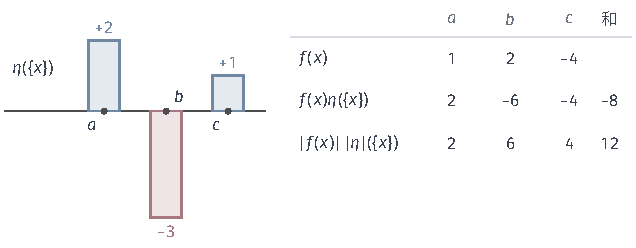
\includegraphics[width=107.692mm]{figures/02-abstract-mathematics/01-metric-and-measure/tikz/c3-signed-measure-masses/figure.pdf}
 \caption{有符号测度$\eta=2\delta_a-3\delta_b+\delta_c$上的积分。左侧柱高为各点质量$\eta(\{x\})$，蓝色为正、红色为负；右表列出$f$的取值、逐点贡献$f(x)\eta(\{x\})$及其和$-8$，以及绝对贡献$|f(x)|\,|\eta|(\{x\})$及其和$12$。}
 \label{fig:integral-signed-measure-masses}
\end{figure}
